% Options for packages loaded elsewhere
\PassOptionsToPackage{unicode}{hyperref}
\PassOptionsToPackage{hyphens}{url}
% !TeX program = pdfLaTeX
\documentclass[12pt]{article}
\usepackage{amsmath}
\usepackage{graphicx,psfrag,epsf}
\usepackage{enumerate}
\usepackage[]{natbib}
\usepackage{textcomp}


%\pdfminorversion=4
% NOTE: To produce blinded version, replace "0" with "1" below.
\newcommand{\blind}{0}

% DON'T change margins - should be 1 inch all around.
\addtolength{\oddsidemargin}{-.5in}%
\addtolength{\evensidemargin}{-1in}%
\addtolength{\textwidth}{1in}%
\addtolength{\textheight}{1.7in}%
\addtolength{\topmargin}{-1in}%

%% load any required packages here



% tightlist command for lists without linebreak
\providecommand{\tightlist}{%
  \setlength{\itemsep}{0pt}\setlength{\parskip}{0pt}}




\IfFileExists{bookmark.sty}{\usepackage{bookmark}}{\usepackage{hyperref}}
\IfFileExists{xurl.sty}{\usepackage{xurl}}{} % add URL line breaks if available
\hypersetup{
  pdftitle={Maximizing Fairness with Synthetic data: Access to Emergency Fund in Sub-Saharan Africa},
  pdfkeywords={Fairness metrics; emergency funds; financial inclusion;
gender-based bias \& debiasing; Sub-Saharan Africa; predictive machine
learning; synthetic data},
  hidelinks,
  pdfcreator={LaTeX via pandoc}}



\begin{document}


\def\spacingset#1{\renewcommand{\baselinestretch}%
{#1}\small\normalsize} \spacingset{1}


%%%%%%%%%%%%%%%%%%%%%%%%%%%%%%%%%%%%%%%%%%%%%%%%%%%%%%%%%%%%%%%%%%%%%%%%%%%%%%

\if0\blind
{
  \title{\bf Maximizing Fairness with Synthetic data: Access to
Emergency Fund in Sub-Saharan Africa}

  \author{
        Charavee Basnet Chettri, Vivian Wei, Betty Pu, Ziyue
Yang \thanks{We are grateful to the Women at the Table team and Sofia
Kypraiou for the project inspiration and suggesting the path forward} \\
    Department of Statistical and Data Sciences, Smith College,
Northampton MA\\
      }
  \maketitle
} \fi

\if1\blind
{
  \bigskip
  \bigskip
  \bigskip
  \begin{center}
    {\LARGE\bf Maximizing Fairness with Synthetic data: Access to
Emergency Fund in Sub-Saharan Africa}
  \end{center}
  \medskip
} \fi

\bigskip
\begin{abstract}
Financial inclusion is paramount for economic stability and resilience,
particularly in diverse regions like Sub-Saharan Africa, spanning low to
high-income countries and encompassing both resource-intensive and
non-resource-intensive economies. This study focuses on a crucial aspect
of financial resilience: the accessibility of emergency funds, defined
as having access to 1/20 of Gross National Income (GNI) per capita in
local currency within 30 days. Leveraging previous colleagues'
exploratory work on the Global Financial Inclusion Database 2021, our
objective is to mitigate inherent gender biases in the dataset by
rebalancing it with synthetic data, thereby enhancing fairness in
predicting emergency fund accessibility. Through predictive machine
learning modeling, we aim to contribute to the economic empowerment of
individuals in Sub-Saharan Africa, ultimately fostering resilience and
reducing disparities in access to essential financial resources.
\end{abstract}

\noindent%
{\it Keywords:} Fairness metrics; emergency funds; financial inclusion;
gender-based bias \& debiasing; Sub-Saharan Africa; predictive machine
learning; synthetic data

\vfill

\newpage
\spacingset{1.9} % DON'T change the spacing!

\hypertarget{introduction}{%
\section{Introduction}\label{introduction}}

In the realm of financial inclusion, the accessibility of emergency
funds plays a pivotal role in determining an individual's financial
stability and resilience, especially in developing countries
\citep{10.1093/oso/9780198827535.003.0007}. In this project, our goal is
to predict the possibility for people in Sub-Saharan African countries
to come up with emergency funds, defined as 1/20 of GNI per capita in
local currency, within a 30-day period\citep{Demirguc-Kunt2022}. This
prediction serves as a crucial factor for establishing future public
financial policies, such as determining the eligibility of individuals
for loans and financial assistance. The significance of this problem
lies within its direct impact on the economic well-being and empowerment
of individuals in developing regions. According to the
\href{https://www.worldbank.org/en/publication/globalfindex}{Global
Financial Inclusion (Global Findex) Database 2021} published by the
World Bank, only a little over half of people over 15 years of age in
developing economies could access extra funds within 30 days if faced
with unexpected expenses \citep{Demirguc-Kunt2022}. Therefore, there is
a pressing need to understand the factors influencing this accessibility
and eliminate inherent bias in the dataset. By delving into this issue,
we not only contribute to enhancing financial inclusion but also aid in
mitigating the different effects of financial shocks on vulnerable
populations.

Defining fairness is essential since the concept itself is relative
among different people. In the data science discourse, fairness
encompasses three key aspects: individual fairness, group fairness, and
causal fairness\citep{Kypraiou2021What}. Individual fairness focuses on
preventing discrimination against individuals with similar relevant
characteristics. This means ensuring that individuals in similar
situations receive similar outcomes from the model, regardless of
irrelevant factors\citep{10.1145/3461702.3462621}. Group fairness aims
to prevent disparities in outcomes for different groups. This ensures
equal opportunities for all groups, regardless of their
membership\citep{10.1145/3442188.3445876}. Causal fairness goes beyond
simply observing disparities and delves into understanding their
underlying causes. It seeks to mitigate these root causes to achieve
fair outcomes within and across groups\citep{plecko2022causal}.

Our previous colleagues conducted analysis using the \textless AI \&
Equality\textgreater{} Human Rights Toolbox and used a Decision Tree
Classifier machine learning model implemented via Python to predict
access to emergency funds with 68\% accuracy. Their work laid a solid
foundation by exploring demographic and financial variables within the
dataset, and assessed the fairness of the decision tree classifier,
particularly concerning gender bias, and then applied various processing
techniques to enhance the fairness of the model\citep{Porta2022}.

Based on their work, our group aims to incorporate synthetic data to
rebalance the dataset, ensuring equitable representations amongst both
genders in the dataset. Our approach aims to consider a broader
selection of machine learning algorithms and mitigate the disparities
the previous colleagues found in the decision tree's classifier's
predictions and enhance fairness with synthetic data, ultimately better
predict access to emergency funds in south-Saharan Africa
countries\citep{SyntheticDataAIEquality}.

\hypertarget{background-on-sub-saharan-region}{%
\subsection{Background on Sub-Saharan
Region}\label{background-on-sub-saharan-region}}

Sub-Saharan Africa is a region characterized by a diverse economic
landscape, encompassing low, lower-middle, and upper-middle-income
countries. Demographically, Sub-Saharan Africa is marked by a rich
tapestry of cultures and a population exceeding 1.2 billion people. This
expansive and diverse demographic landscape includes 22 countries
grappling with fragility or conflict, posing unique challenges to
development efforts. Additionally, 13 small states within the region are
characterized by limited human capital, modest populations, and
constrained land areas {[}ADD CITATION{]}.

\begin{figure}
\centering
\includegraphics[width=\textwidth,height=0.5\textheight]{images/access_by_educ_level.png}
\caption{Access to Emergency Funds by Education Level}
\end{figure}

\begin{center}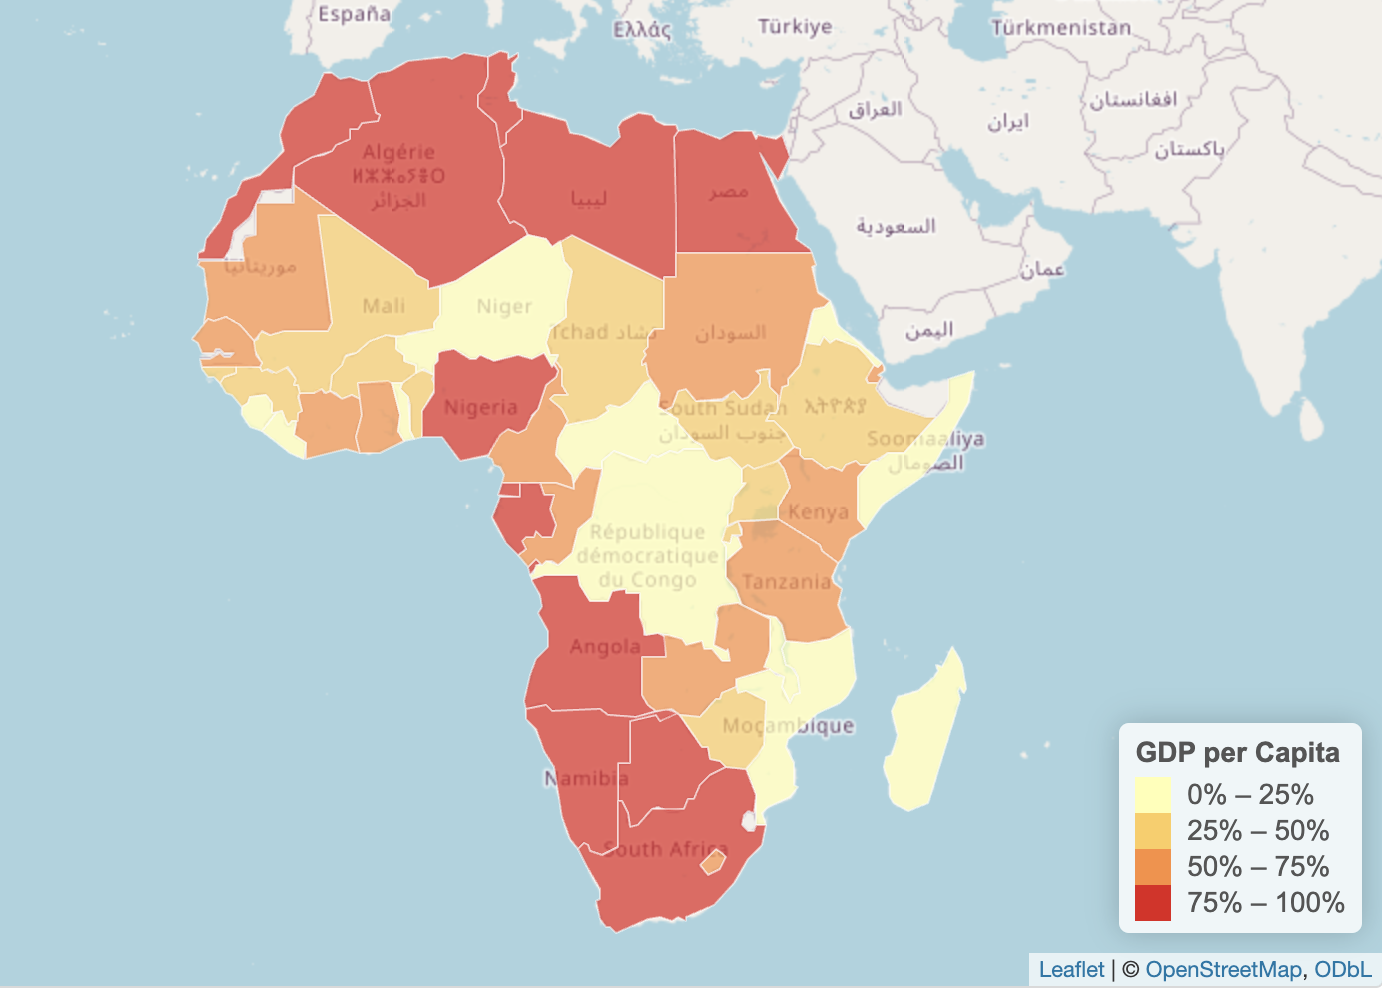
\includegraphics[width=0.7\linewidth]{graphs/map} \end{center}

According to the World Bank's definition, middle-income countries had a
per capita gross national income of more than US\$995.00 in the years
2015--17 {[}ADD CITATION{]}. Among the 35 countries included in our
dataset, 20 are classified as low-income countries, and 15 are
classified as middle-income countries. Additionally, 11 are classified
as countries in Fragile and Conflict-Affected Situations, which, by
definition, have experienced a peacekeeping or peace-building mission
within the last three years.

Sub-Saharan African countries not only differ in terms of economic
prosperity but also in economic structure and resource intensity.
Resource-intensive countries include both oil-exporting nations, where
net oil exports make up 30 percent or more of total exports, and
commodity exporters, where nonrenewable natural resources represent 25
percent or more of total exports. The divergence between
resource-intensive and non-resource-intensive countries became more
entrenched following the commodity price shock of 2015 {[}ADD
CITATION{]}. Non-resource-intensive countries have proven more
resilient, supported by their more diversified economies. On the other
hand, resource-intensive economies generally have a less diversified
structure, making them more susceptible to external shocks. In our
dataset, 6 of the countries are oil exporters, and 11 export other
commodities such as iron ore, copper, cotton, coffee, and sugar. The
remaining 18 countries are non-resource-intensive and their economies
are not reliant on exports.

In recent years, the Sub-Saharan Africa region has grappled with
significant economic challenges, including soaring inflation, pronounced
exchange rate pressures, debt vulnerabilities, and widening economic
disparities within the region. Therefore, addressing these structural
and economic disparities is imperative for tackling developmental issues
in the region.

\hypertarget{data}{%
\section{Data}\label{data}}

In order to continue assessing and enhancing the fairness of the machine
learning models, we use the same Global Findex Database as our
colleagues before us. The Global Findex database was first launched in
2011 by the World Bank---with funding from the Bill \& Melinda Gates
Foundation. It is the world's most comprehensive data set on how adults
save, borrow, make payments, and manage risk. The dataset contains over
200 indicators including account ownership, payments, savings, credit,
and financial resilience and has coverage over 140 nations, representing
97\% of the world's population for year 2017, 2014, and 2011.

The data was constructed through a series of surveys carried out by
Gallup, Inc in association with the annual Gallup World Poll. They
randomly sampled 1000 individuals from each country and asked them to
respond to a survey either over the phone or in-person. The target
population is the civilian, non-institutionalized population 15 years
and above. In consistency with the former colleagues, our sample covers
only the Sub-Saharan region (35 countries total), thus there are 35,000
total observations and 105 total variables. Since the sampling was
random and the sample size is large, we can assume that our sample is
representative of the total population of people living in the 35
Sub-Saharan countries in the data. The data was collected directly from
individuals over the 2017 calendar year and is self-contained, meaning
it does not rely on any external resources.

\hypertarget{variable-definition-and-descriptions}{%
\subsection{Variable Definition and
Descriptions}\label{variable-definition-and-descriptions}}

After basic data cleaning, we have created various visualizations to
help understand who is in the data and acknowledge potential sources of
bias within the data.

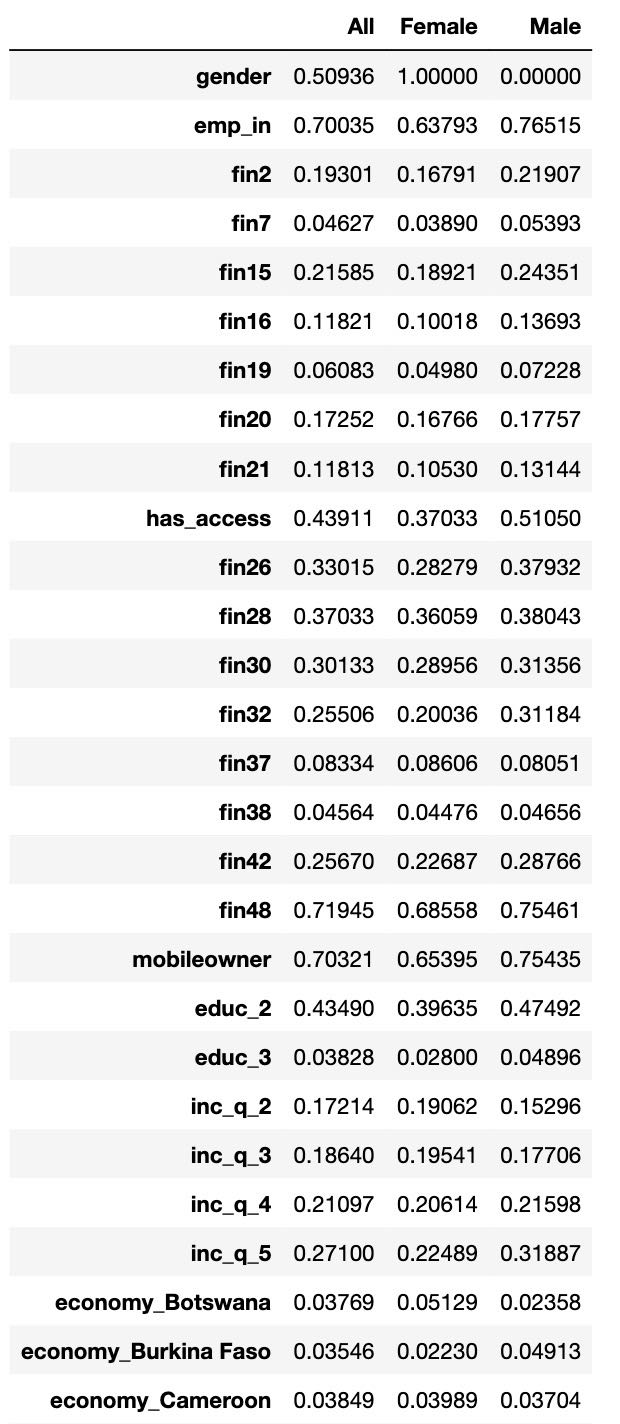
\includegraphics[width=0.4\linewidth]{graphs/var1_graph}
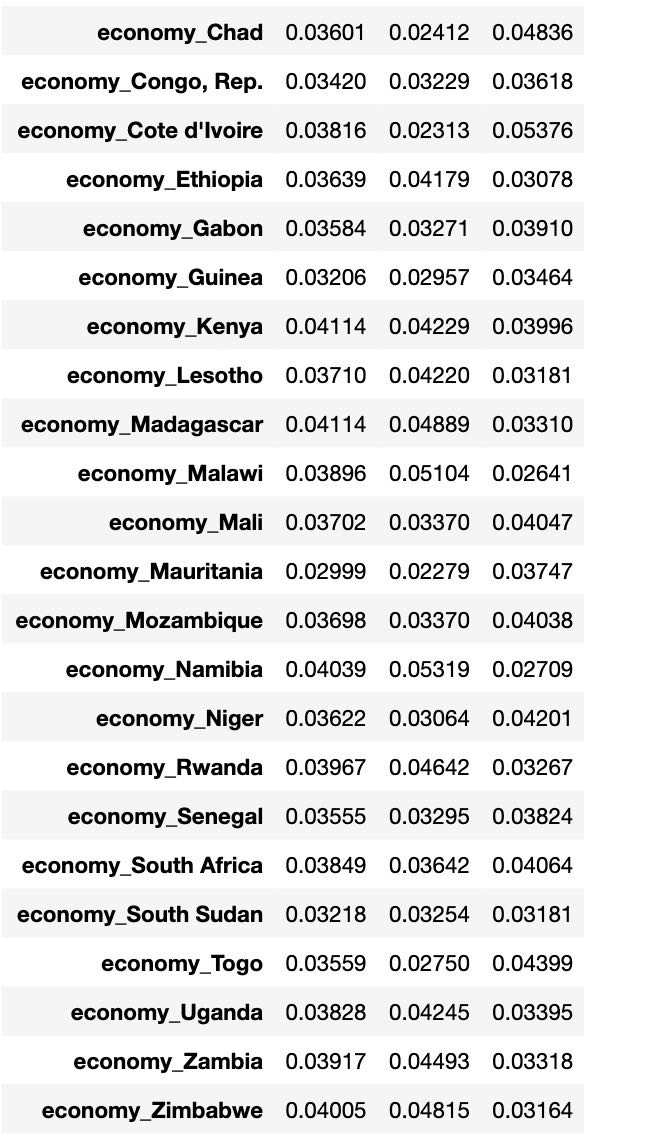
\includegraphics[width=0.4\linewidth]{graphs/var2_graph}

\hypertarget{outcome-variable-of-interest-access-to-emergency-fund-fin24}{%
\subsubsection{\texorpdfstring{\emph{Outcome Variable of Interest:
Access to Emergency Fund
(Fin24)}}{Outcome Variable of Interest: Access to Emergency Fund (Fin24)}}\label{outcome-variable-of-interest-access-to-emergency-fund-fin24}}

The variable ``Fin24'' in the dataset asked participants the question:
Now, imagine that you have an emergency and you need to pay {[}1/20 of
GNI per capita in local currency{]}. Is it possible or not possible that
you could come up with {[}1/20 of GNI per capita in local currency{]}
within the NEXT MONTH? In order to make it more straightforward for
interpretations, we restrict the response into a binary variable for Yes
and No.~The overall distribution of access to emergency funds showed 17,
599 individuals had access to emergency funds while 14342 did not. This
indicates that over half of individuals represented in the data do not
have access to emergency funds.

To help conceptually understand how the outcome variables might vary
among different levels of the variables, we chose 50\% as the benchmark
proportion for checking if the possibility of coming up with emergency
funds for each variable group of interest is different from a random
50/50 chance.

\begin{figure}

{\centering 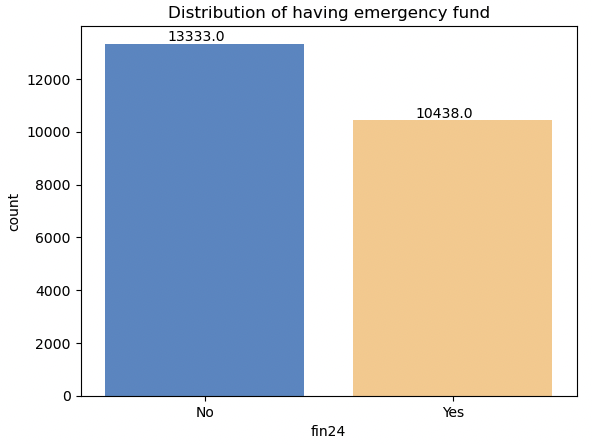
\includegraphics[width=0.7\linewidth]{graphs/f24_graph1} 

}

\caption{Distribution of having emergency fund}\label{fig:unnamed-chunk-4}
\end{figure}

\hypertarget{protected-attribute-of-focus-gender-female}{%
\subsubsection{\texorpdfstring{\emph{Protected Attribute of Focus:
Gender
(female)}}{Protected Attribute of Focus: Gender (female)}}\label{protected-attribute-of-focus-gender-female}}

The variable ``female'' distinguishes gender. There are 12108 females
and 11663 males in the dataset. It appears to have a fair distribution
between different genders for the dataset as a whole.

\begin{figure}

{\centering 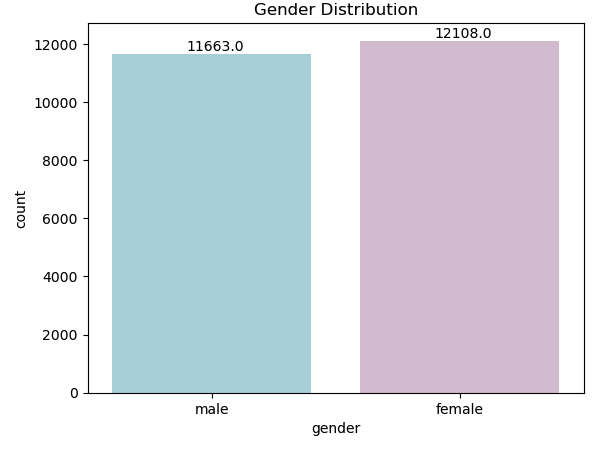
\includegraphics[width=1\linewidth]{graphs/f24_graph2} 

}

\caption{Distribution on gender}\label{fig:unnamed-chunk-5}
\end{figure}

While it looks quite balanced in the previous figure, we observe a
discrepancy between the two genders when compared against our outcome
variable of interest. Females have a 15\% lower chance of having access
to emergency funds.

\begin{figure}

{\centering 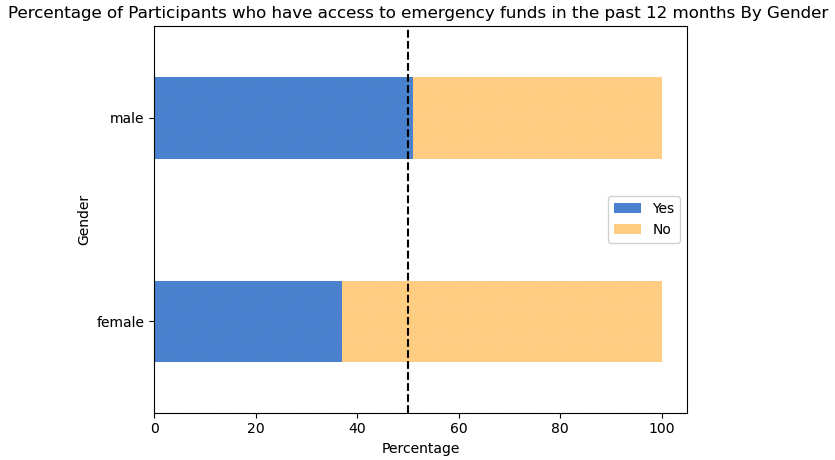
\includegraphics[width=1\linewidth]{graphs/f24_graph3} 

}

\caption{Distribution of having emergency fund by gender}\label{fig:unnamed-chunk-6}
\end{figure}

In order to investigate further into how discrepancy of gender plays
into other predictor variables, we created visuals for contrasting the
two genders.

\hypertarget{education-educ}{%
\subsubsection{\texorpdfstring{\emph{Education
(educ)}}{Education (educ)}}\label{education-educ}}

The variable ``educ'' distinguishes education level among participants:
1 being the completed primary education or less, 2 being completed
secondary education, and 3 being completed tertiary education. The
majority in the dataset is participants with primary or less education
(12523 participants). On the other hand, there are only 910 participants
who have tertiary education. Overall, the discrepancy between education
levels appears quite drastic, and might result in a varying prediction
for access to emergency funds. If we break down education by gender, we
see that more females than males have primary or less education while
the opposite for secondary or tertiary education.

\begin{figure}

{\centering 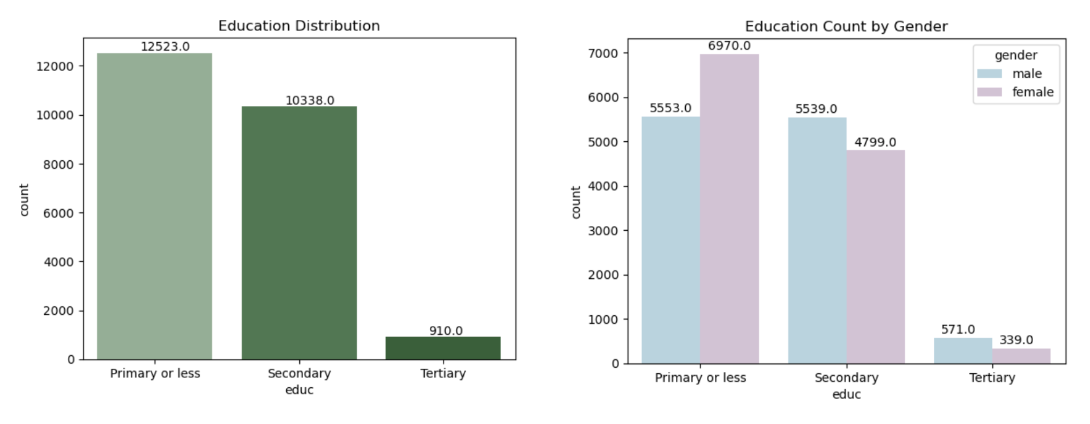
\includegraphics[width=1\linewidth]{graphs/f24_graph4} 

}

\caption{Distribution by education level}\label{fig:unnamed-chunk-7}
\end{figure}

When we consider gender and education with respect to the outcome
variable of interest, we observe that tertiary education levels have the
highest likelihood of access to emergency funds while primary education
is the least likely.

\begin{figure}

{\centering 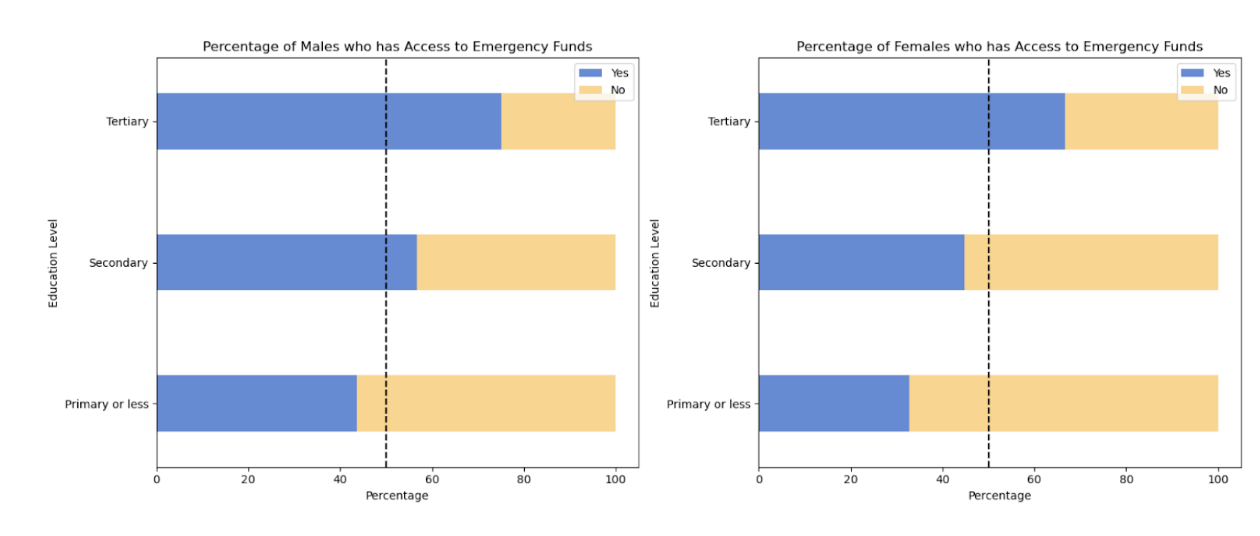
\includegraphics[width=1\linewidth]{graphs/f24_graph5} 

}

\caption{Distribution of access to emergency funds by education level and gender}\label{fig:unnamed-chunk-8}
\end{figure}

This discrepancy between education levels is reasonable since
participants with tertiary education might have been more financially
independent and have higher financial resilience, thus be more likely to
have access to emergency funds. Nonetheless, we continue to observe that
females have a lower access to emergency funds, among the same education
level. It shows that gender imbalance is still evident when we position
it in relationship to other predictors.

\hypertarget{income-quantile-inc_q}{%
\subsubsection{\texorpdfstring{\emph{Income Quantile
(Inc\_q)}}{Income Quantile (Inc\_q)}}\label{income-quantile-inc_q}}

The variable ``inc\_q'' distinguishes the income quintile within an
economy. It is separated into 5 quantiles with 1 being the poorest and 5
being the richest. Income quintile 5, or the richest 20\%, is the
largest quantile. There are more male than females in the richest 20\%
quintile, while females compose the majority of the poorest 20\%, second
poorest 20\%, and middle 20\%, which are the poorest quantiles.

\begin{figure}

{\centering 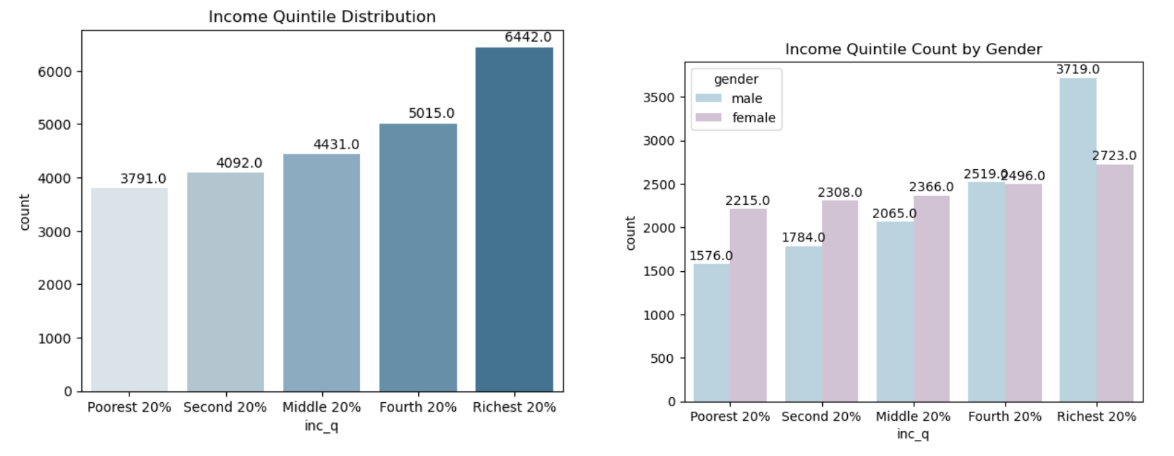
\includegraphics[width=1\linewidth]{graphs/income_graph6} 

}

\caption{Income Quantile Distribution}\label{fig:unnamed-chunk-9}
\end{figure}

We observe a similar gradient in access to emergency funds among the
different income quintiles. This discrepancy is expected since
participants with the level of income are directly related to financial
stability and resilience. However, the gap between females and male is
still concerning: male that are in the top two income quintile will have
at least 50\% chance of access to emergency funds, whereas only females
that are the top 1 income quintile will have a comparable likelihood.

\begin{figure}

{\centering 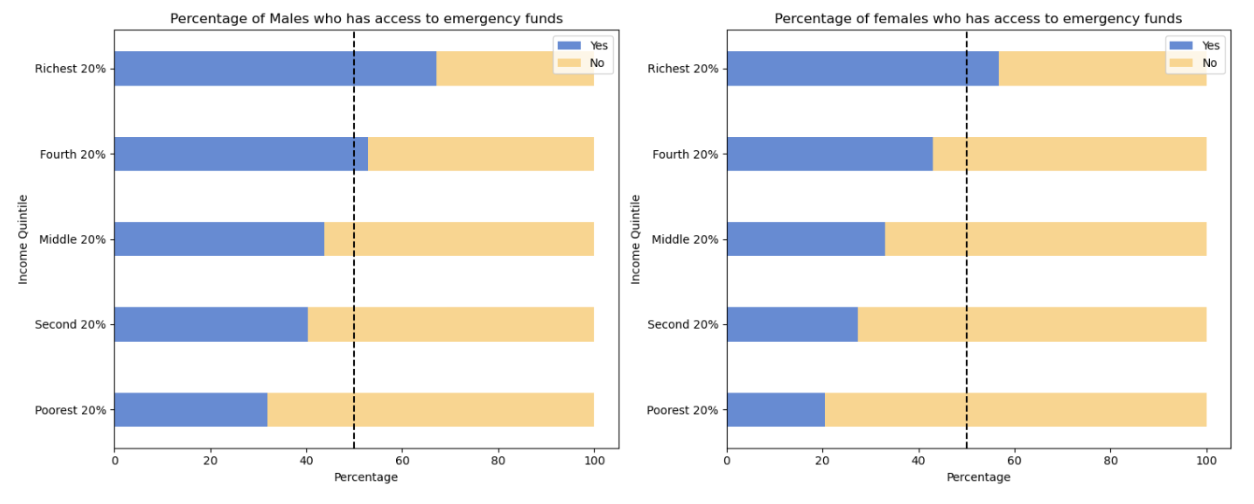
\includegraphics[width=1\linewidth]{graphs/employ_graph7} 

}

\caption{Distribution of access to emergency funds by income quantiile and gender}\label{fig:unnamed-chunk-10}
\end{figure}

\hypertarget{employment-status-emp_in}{%
\subsubsection{\texorpdfstring{\emph{Employment Status
(emp\_in)}}{Employment Status (emp\_in)}}\label{employment-status-emp_in}}

Employment Status asks whether or not the participant is in the
workforce. There are 16648 individuals who were in the workforce while
7123 were not, and more females are out of the workforce than males,
thus suggesting that females are less likely to achieve economic
independence than males.

\begin{figure}

{\centering 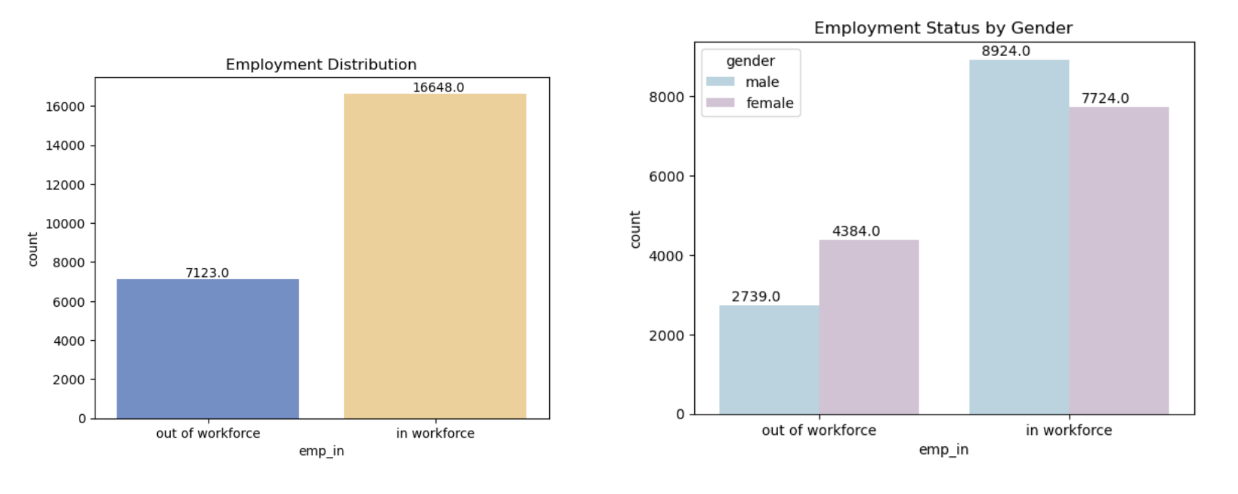
\includegraphics[width=1\linewidth]{graphs/employ_graph8} 

}

\caption{Distribution of employment status}\label{fig:unnamed-chunk-11}
\end{figure}

The disparity between females and male is quite alarming when we break
it down by employment status. Regardless of the employment status,
females do not even have a 50\% chance of having access to emergency
funds.

\begin{figure}

{\centering 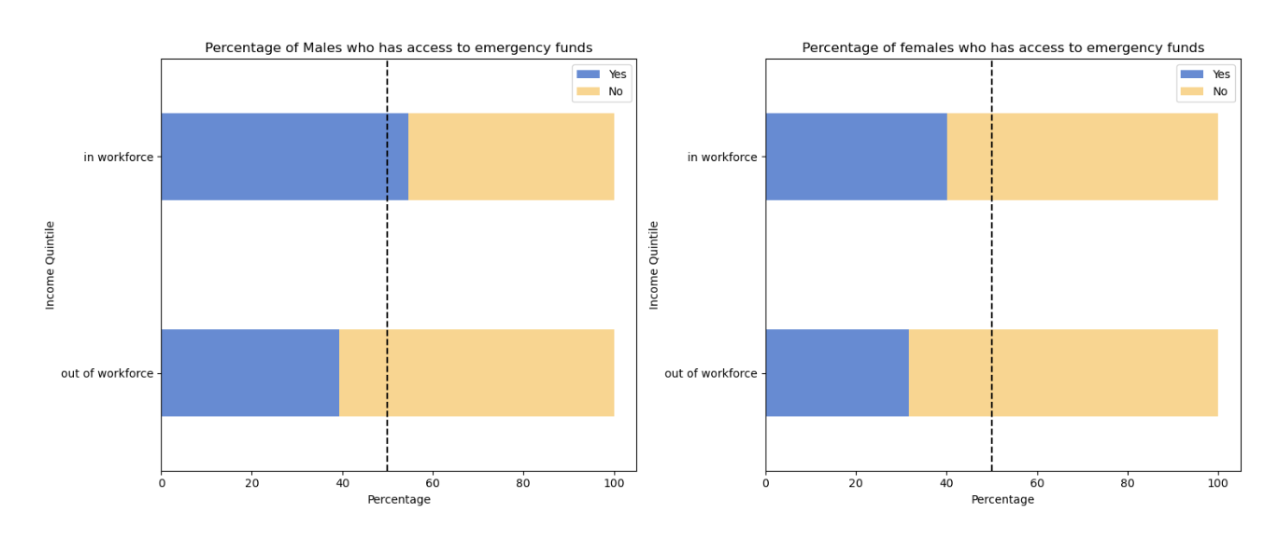
\includegraphics[width=1\linewidth]{graphs/employ_graph9} 

}

\caption{Distribution of access to emergency funds by employment status and gender}\label{fig:unnamed-chunk-12}
\end{figure}

\hypertarget{country-economy}{%
\subsubsection{\texorpdfstring{\emph{Country
(economy)}}{Country (economy)}}\label{country-economy}}

The ``economy'' variable represents the country that the participants
live in. There are 27 different countries from Sub-Saharan Africa with
around 800-900 respondents each. The countries included are Benin,
Botswana, Burkina Faso, Cameroon, Central African Republic, Chad, Congo
Dem. Rep.~Congo Rep., Côte d'Ivoire, Ethiopia, Gabon, Ghana, Guinea,
Kenya, Lesotho, Liberia, Madagascar, Malawi, Mali, Mauritania,
Mozambique, Namibia, Niger, Nigeria, Rwanda, Senegal, Sierra Leone,
South Africa, South Sudan, Tanzania, Togo, Uganda, Zambia, and Zimbabwe.

While looking at the outcome variable of interest broken down by country
and gender, we see that Liberia has the highest proportion of both
females and male having access to emergency funds, while Zambia has the
lowest proportion of accessing emergency funds in both females and
males. It's also important to note that the difference between males and
females is largest in countries like Botswana and Kenya.

\begin{figure}

{\centering 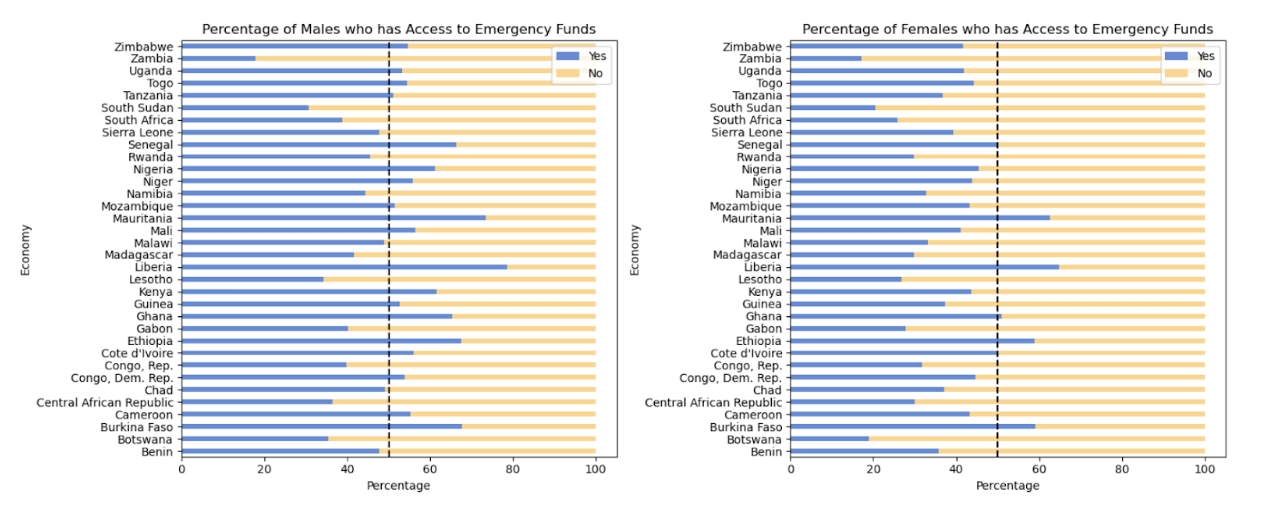
\includegraphics[width=1\linewidth]{graphs/country_graph10} 

}

\caption{Distributions of Access to Emergency Funds by country and gender}\label{fig:unnamed-chunk-13}
\end{figure}

We iterate the visualizations for each main financial variable of
interest in the dataset by gender, by gender and economy, and by gender
and education level, to check if there's recurring discrepancy among
genders. Due to the page constraints, we decide to not include all
visualizations and attach our
\href{https://drive.google.com/file/d/1f9AauOn4I2Rl5io_viMw0WbEXKFiJcRA/view?usp=sharing}{Jupyter
Notebook} for reference.

\bibliographystyle{plain}
\bibliography{bibliography.bib}



\end{document}
